\documentclass{article}

\usepackage{tikz}
\usetikzlibrary{arrows.meta}

\definecolor{navy}{RGB}{20,55,100}
\definecolor{steel}{RGB}{70,100,130}
\definecolor{red}{RGB}{190,60,60}
\definecolor{redpale}{RGB}{255,235,235}
\definecolor{gold}{RGB}{190,140,40}
\definecolor{goldpale}{RGB}{255,248,220}
\definecolor{green}{RGB}{45,140,85}
\definecolor{greenpale}{RGB}{230,248,238}
\definecolor{bluepale}{RGB}{235,242,250}

\begin{document}
	
	\begin{figure}[ht]
		\centering
		
		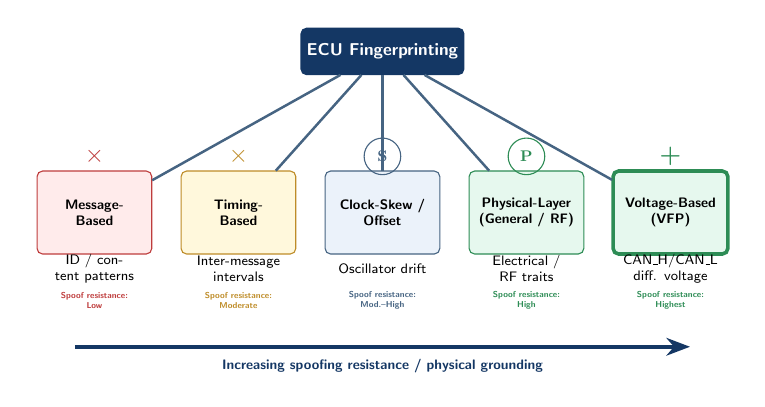
\begin{tikzpicture}[scale=0.62, transform shape]
			
			% ROOT
			\node[
			rectangle,
			rounded corners=2pt,
			draw=navy,
			fill=navy,
			text=white,
			minimum width=3.3cm,
			minimum height=0.95cm,
			align=center,
			font=\sffamily\bfseries
			] (root) at (5.9,3.3)
			{ECU Fingerprinting};
			
			% MESSAGE BASED
			\node[
			rectangle,
			rounded corners=2pt,
			draw=red,
			fill=redpale,
			minimum width=2.35cm,
			minimum height=1.7cm,
			align=center,
			font=\sffamily\bfseries\footnotesize
			] (a) at (0,0)
			{\textbf{Message-}\\\textbf{Based}};
			
			% TIMING BASED
			\node[
			rectangle,
			rounded corners=2pt,
			draw=gold,
			fill=goldpale,
			minimum width=2.35cm,
			minimum height=1.7cm,
			align=center,
			font=\sffamily\bfseries\footnotesize
			] (b) at (2.95,0)
			{\textbf{Timing-}\\\textbf{Based}};
			
			% CLOCK SKEW
			\node[
			rectangle,
			rounded corners=2pt,
			draw=steel,
			fill=bluepale,
			minimum width=2.35cm,
			minimum height=1.7cm,
			align=center,
			font=\sffamily\bfseries\footnotesize
			] (c) at (5.9,0)
			{\textbf{Clock-Skew /}\\\textbf{Offset}};
			
			% PHYSICAL LAYER
			\node[
			rectangle,
			rounded corners=2pt,
			draw=green,
			fill=greenpale,
			minimum width=2.35cm,
			minimum height=1.7cm,
			align=center,
			font=\sffamily\bfseries\footnotesize
			] (d) at (8.85,0)
			{\textbf{Physical-Layer}\\\textbf{(General / RF)}};
			
			% VOLTAGE BASED
			\node[
			rectangle,
			rounded corners=2pt,
			draw=green,
			fill=greenpale,
			line width=1.3pt,
			minimum width=2.35cm,
			minimum height=1.7cm,
			align=center,
			font=\sffamily\bfseries\footnotesize
			] (e) at (11.8,0)
			{\textbf{Voltage-Based}\\\textbf{(VFP)}};
			
			% ICONS
			\node[
			font=\Large\bfseries,
			text=red
			] at (0,1.15) {$\times$};
			
			\node[
			font=\Large\bfseries,
			text=gold
			] at (2.95,1.15) {$\times$};
			
			\node[
			draw=steel,
			circle,
			minimum size=0.75cm,
			text=steel,
			font=\small\bfseries
			] at (5.9,1.15) {S};
			
			\node[
			draw=green,
			circle,
			minimum size=0.75cm,
			text=green,
			font=\small\bfseries
			] at (8.85,1.15) {P};
			
			\node[
			font=\Large\bfseries,
			text=green
			] at (11.8,1.15) {+};
			
			% CONNECTION LINES
			\draw[draw=steel, line width=0.9pt]
			(root) -- (a);
			
			\draw[draw=steel, line width=0.9pt]
			(root) -- (b);
			
			\draw[draw=steel, line width=0.9pt]
			(root) -- (c);
			
			\draw[draw=steel, line width=0.9pt]
			(root) -- (d);
			
			\draw[draw=steel, line width=0.9pt]
			(root) -- (e);
			
			% DESCRIPTIONS
			\node[
			font=\sffamily\footnotesize,
			align=center,
			text width=2.5cm
			] at (0,-1.15)
			{ID / content patterns};
			
			\node[
			font=\sffamily\footnotesize,
			align=center,
			text width=2.5cm
			] at (2.95,-1.15)
			{Inter-message intervals};
			
			\node[
			font=\sffamily\footnotesize,
			align=center,
			text width=2.5cm
			] at (5.9,-1.15)
			{Oscillator drift};
			
			\node[
			font=\sffamily\footnotesize,
			align=center,
			text width=2.5cm
			] at (8.85,-1.15)
			{Electrical / RF traits};
			
			\node[
			font=\sffamily\footnotesize,
			align=center,
			text width=2.5cm
			] at (11.8,-1.15)
			{CAN\_H/CAN\_L diff. voltage};
			
			% SPOOFING RESISTANCE
			\node[
			font=\tiny\bfseries\sffamily,
			text=red,
			align=center
			] at (0,-1.8)
			{Spoof resistance:\\Low};
			
			\node[
			font=\tiny\bfseries\sffamily,
			text=gold,
			align=center
			] at (2.95,-1.8)
			{Spoof resistance:\\Moderate};
			
			\node[
			font=\tiny\bfseries\sffamily,
			text=steel,
			align=center
			] at (5.9,-1.8)
			{Spoof resistance:\\Mod.--High};
			
			\node[
			font=\tiny\bfseries\sffamily,
			text=green,
			align=center
			] at (8.85,-1.8)
			{Spoof resistance:\\High};
			
			\node[
			font=\tiny\bfseries\sffamily,
			text=green,
			align=center
			] at (11.8,-1.8)
			{Spoof resistance:\\Highest};
			
			% BOTTOM ARROW
			\draw[
			-{Stealth[length=3mm]},
			line width=1.3pt,
			draw=navy
			] (-0.4,-2.75) -- (12.2,-2.75);
			
			\node[
			font=\sffamily\bfseries\footnotesize,
			text=navy,
			align=center
			] at (5.9,-3.15)
			{Increasing spoofing resistance / physical grounding};
			
		\end{tikzpicture}
		
		\caption{ECU Fingerprinting Methods: From Message-Based to Voltage-Based Identification.}
		
		\label{fig:fp_taxonomy}
		
	\end{figure}
	
\end{document}